\documentclass[11pt,a4paper]{article}
\usepackage{url}
\usepackage{color}
\usepackage{graphicx}
\usepackage{cjhebrew}
\usepackage[T2A,OT2,OT1]{fontenc}
\usepackage{ucs}
\usepackage{CJKutf8}

\usepackage{subfigure}
\usepackage{floatrow}
\usepackage{multirow}
\usepackage[hebrew,english]{babel}

\usepackage{times}
\usepackage{latexsym}
\usepackage{acl2014}
\usepackage[small]{caption}

\newcommand{\heb}[1]{%
  \foreignlanguage{hebrew}{#1} }

\newcommand\cyr{%
\renewcommand\rmdefault{wncyr}% \renewcommand\sfdefault{wncyss}%
\renewcommand\encodingdefault{OT2}%
\normalfont
\selectfont}
\DeclareTextFontCommand{\textcyr}{\cyr}

\newcommand{\ddcomment}[1]{\textcolor{red}{[$^{\textsc{D}}_{\textsc{D}}$ #1]}}
\newcommand{\spcomment}[1]{\textcolor{blue}{[$^{\textsc{S}}_{\textsc{P}}$ #1]}}
\newcommand{\jmcomment}[1]{\textcolor{magenta}{[$^{\textsc{J}}_{\textsc{M}}$ #1]}}
\newcommand{\eat}[1]{\ignorespaces}

\newcommand{\query}[1]{\texttt{#1}}

\setlength\titlebox{6.5cm}    % Expanding the titlebox

\title{Enhanced Search with Wildcards and Morphological Inflections\\in the Google Books Ngram Viewer}

\eat{\author{Jason Mann, David Zhang, Lucille Yang, Slav Petrov and Dipanjan Das\\
	Google Inc. \\
	{\tt jcm2207@columbia.edu, dzhang21@gmail.com, ly77@cornell.edu}\\
	{\tt \{slav,dipanjand\}@google.com}}
}

\date{}

\begin{document}
\maketitle

\begin{abstract}

We present a new version of the Google Books Ngram Viewer, which plots
the frequency of words and phrases over the last five
centuries; its data encompasses 6\% of the world's published books.
The new Viewer adds three features for more powerful search: wildcards,
morphological inflections, and capitalization. These additions allow
the discovery of patterns that were previously difficult to find in the Google Books Ngram data,
and further facilitate the study of linguistic trends in printed text.

\end{abstract}

\section{Introduction}

The Google Books Ngram project facilitates the analysis of cultural, social and linguistic trends through five centuries of written text in eight languages. The Ngram Corpus \cite{culturomics,lin2012syntactic} consists of words and phrases (i.e., ngrams) and their usage frequency over time; it is freely available for download. The interactive Ngram Viewer\footnote{See \url{http://books.google.com/ngrams}.} allows users to retrieve and plot the frequency of multiple ngrams on a simple webpage. The Viewer is widely popular and can be used to efficiently explore and visualize patterns in the underlying ngram data. For example, the ngram data has been used to detect emotion trends in 20th century books \cite{acerbi.etal.2013}, to analyze text focusing on market capitalism throughout the past century \cite{Schulz2013}, detect social and cultural impact of historical personalities \cite{skiena.ward.2013}, or to analyze the correlation of economic crises with a literary `misery index' reflected in printed text during crises periods \cite{bentley.et.al.2014}.

\begin{figure}[t]
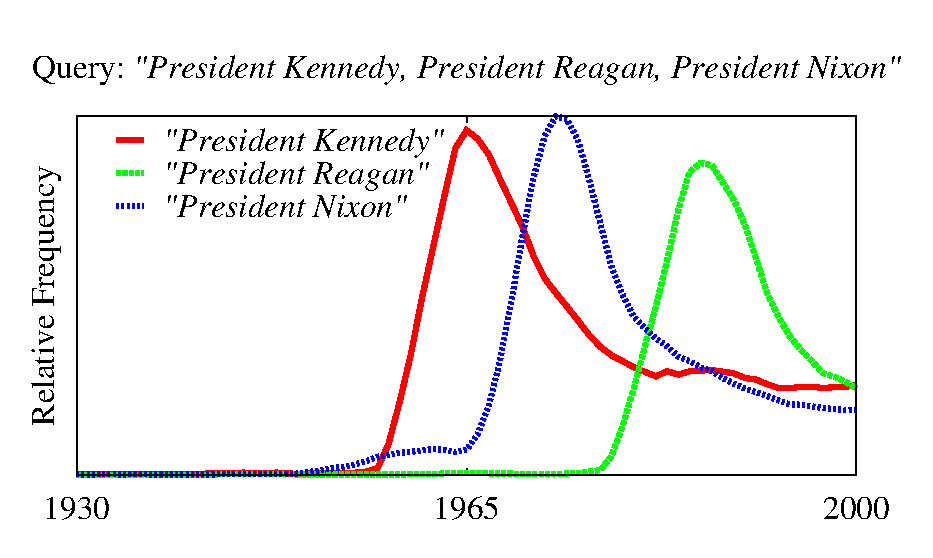
\includegraphics[width=\columnwidth]{graphs/kenreanixon}
\caption{\label{fig:manual}Mention frequencies for three different American presidents queried one-by-one.
\vspace{-1.5em}}
\end{figure}

A limitation of the Viewer, however, is that all the reasoning has to be done by the user, and only individual, user-specified ngrams can be retrieved and plotted. For example, to compare the popularity of different presidents, one needs to come up with a list of presidents and then search for them one-by-one. The result of the query `\query{President Kennedy, President Nixon, President Reagan}' is shown in Figure~\ref{fig:manual}. To determine the most popular president, one would need to search for all presidents, which is cumbersome and should ideally be automated.



In this paper, we therefore present an updated version of the Viewer that enhances its search functionality. We introduce three new features that automatically expand a given query and retrieve a collection of ngrams, to facilitate the discovery of patterns in the underlying data. First, users can replace one query term with a placeholder symbol `\query{*}' (wildcard, henceforth), which will return the ten most frequent expansions of the wildcard in the corpus for the specified year range. 
%Figure~\ref{fig:examples}(a) shows the automatically discovered increase in references to the University of California. 
Second, by adding a specific marker to any word in a query (`\query{\_INF}'), ngrams with all morphological inflections of that word will be retrieved. 
%Figure~\ref{fig:examples}(b) shows the four inflected forms of the word book in the ngram `book a hotel'.
Finally, the new Viewer supports capitalization searches, which return all capitalization variants of the query ngram. Figure~\ref{fig:examples} provides examples for these three new types of queries.
%Figure~\ref{fig:examples}(c) shows the decline in the camel-case spelling of the surname Fitzgerald.
% Slav: we could discuss the examples in Fig. 1 here.

While it is fairly obvious how the above search features can be implemented via brute-force computation, supporting an interactive application with low latency necessitates some non-trivial engineering. In particular, the wildcard search feature poses some challenges because the most frequent expansions depend on the selected year range (consider the frequency with which presidents are mentioned during different decades, for example). To this end, we provide details on our system architecture in \S\ref{sec:overview}  and discuss how the new search features are implemented in \S\ref{sec:features}.
% We could add a sentence summarizing how we deal with wildcards here.


\begin{figure}[!t]
\begin{subfigure}
  \centering
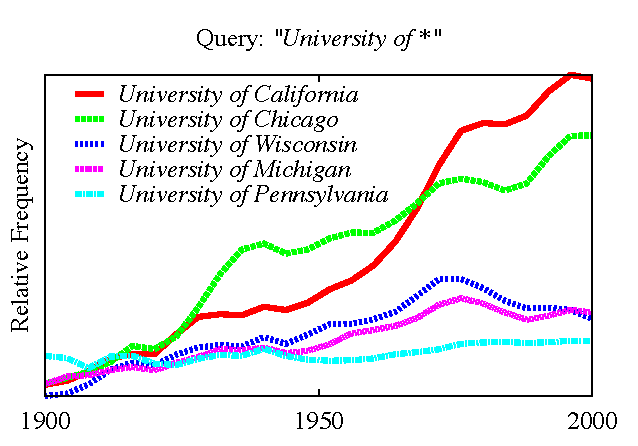
\includegraphics[width=\columnwidth]{graphs/university}\\
\end{subfigure}%
\vspace{-1em}
\begin{subfigure}
\centering
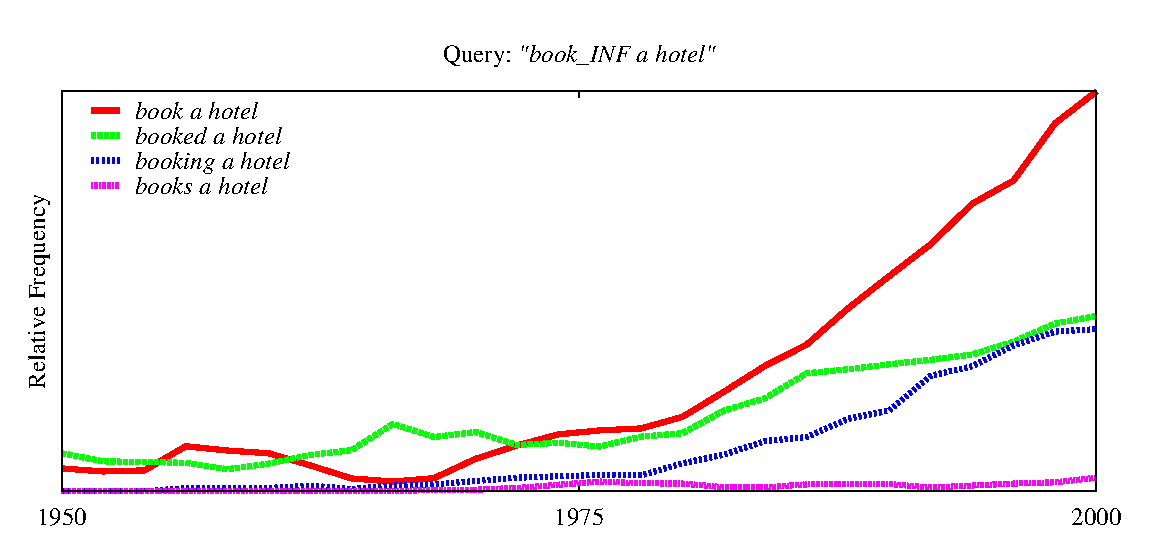
\includegraphics[width=\columnwidth]{graphs/book}\\
\end{subfigure}%
\vspace{-1em}
\begin{subfigure}
\centering
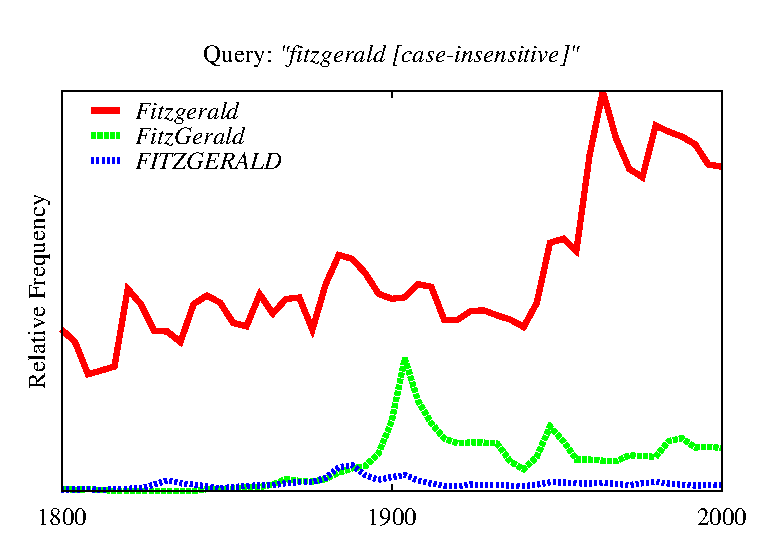
\includegraphics[width=\columnwidth]{graphs/fitzgerald}\\
\end{subfigure}
\caption{In the new enhanced search features of the Ngram Viewer presented here, a single query is automatically expanded to retrieve multiple related ngrams. From top to bottom, we show examples of the wildcard operator (`\query{*}'), the `\query{\_INF}' marker that results in morphological inflections, and the case insensitive search functionality. \label{fig:examples} We show fewer results in this figure than the ones returned by the Ngram Viewer due to space considerations.
\vspace{-1.5em}}
\vspace{-1em}
\end{figure}

In addition, we present an overhaul of the Ngram Viewer's user interface with interactive features that allow for easier management of the increase in data points returned (\S\ref{sec:usecases}). \eat{For example, to normalize for morphological inflections or casing, the frequencies of multiple ngrams can be aggregated via a (right) mouse-click. Additionally, lines can be highlighted or faded (via hovering or mouse-clicks) to focus on particular ngrams and make trends more apparent.} We emphasize that this demonstration updates only the Viewer, and provides tools for easier analysis of the underlying corpora. The ngram corpora themselves are not updated.
Detailed analysis and interpretation of trends uncovered with the new search interface is beyond the scope of this paper. We focus on some interesting use cases in \S\ref{sec:usecases}; many of the presented queries were difficult (or impossible) to execute in the previous versions of the system.

\section{System Overview}
\label{sec:overview}

We start by presenting an overview of the system architecture. We briefly review the underlying corpus and architecture of previous versions of the Viewer \cite{culturomics,lin2012syntactic} and then focus on the extensions added in this version.


\subsection{The Ngram Corpus}
	The Google Books Ngram Corpus\footnote{Downloadable from \texttt{https://books.google.com/} \texttt{ngrams/datasets}.} provides ngram counts for eight different languages over more than 500 years; additionally, the English corpus is split further into British vs. American English and Fiction to aid domain restriction. This corpus is a subset of all books digitized at Google, and represents more than 6\% of all publicized texts \cite{lin2012syntactic}. Two editions of the corpus are available: the first edition dates from 2009 and is described in \newcite{culturomics}; the second edition is from 2012 and is described in \newcite{lin2012syntactic}. The new search features presented here are available for both editions.

\newcite{culturomics} extract ngrams for each page in isolation. More specifically, they use whitespace tokenization and extract all ngrams up to length five. These ngrams include ngrams that potentially span sentence boundaries, but do not include ngrams that span across page breaks (even when they are part of the same sentence).
\newcite{lin2012syntactic} on the other hand perform tokenization, text normalization and segmentation into sentences. They then add synthetic \textsf{\textsc{\_start\_}} and \textsf{\textsc{\_end\_}} tokens to the beginning and end of the sentences to enable the distinction of sentence medial ngrams from those near sentence boundaries \cite{lin2012syntactic}. They also make sure to include sentences that span across page boundaries. Due to these differences, as well as the availability of additional book data, improvements to the optical character recognition algorithms and metadata extraction for dating the books, the ngrams counts from the two editions are not the same.

The edition from \newcite{lin2012syntactic} additionally includes syntactic ngrams. The corpus is tagged using the universal part-of-speech (POS) tag set of \newcite{petrov2012universal}: \query{NOUN} (nouns), \query{VERB} (verbs), \query{ADJ} (adjectives), \query{ADV} (adverbs), \query{PRON} (pronouns), \query{DET} (determiners and articles), \query{ADP} (prepositions and postpositions), \query{CONJ} (conjunctions). Words can be disambiguated by their POS tag by simply appending the tag to the word with an underscore (e.g. \texttt{book\_NOUN}) and can also be replaced by POS tags in the ngrams, see \newcite{lin2012syntactic} for details. The corpus is  parsed with a dependency parser and head-modifier syntactic relations between words in the same sentence are extracted. Dependency relations are represented as `\query{=>}' in the corpus. Our new enhanced search features for automatic expansions can also be applied to these syntactic ngrams. In fact, some of the most interesting queries use expansions to automatically uncover related ngrams, while using syntax to focus on particular patterns.

The Viewer supports the composition of ngram frequencies via arithmetic operators. Addition (\query{+}), subtraction (\query{-}) and division (\query{/}) of ngrams are carried out on a per year basis, while multiplication (\query{*}) is performed by a scalar that is applied to all counts in the time series. Where ambiguous, the wildcard operator takes precedence over the multiplication operator. Parentheses can be used to disambiguate and to force a particular interpretation.

\begin{figure}[!t]
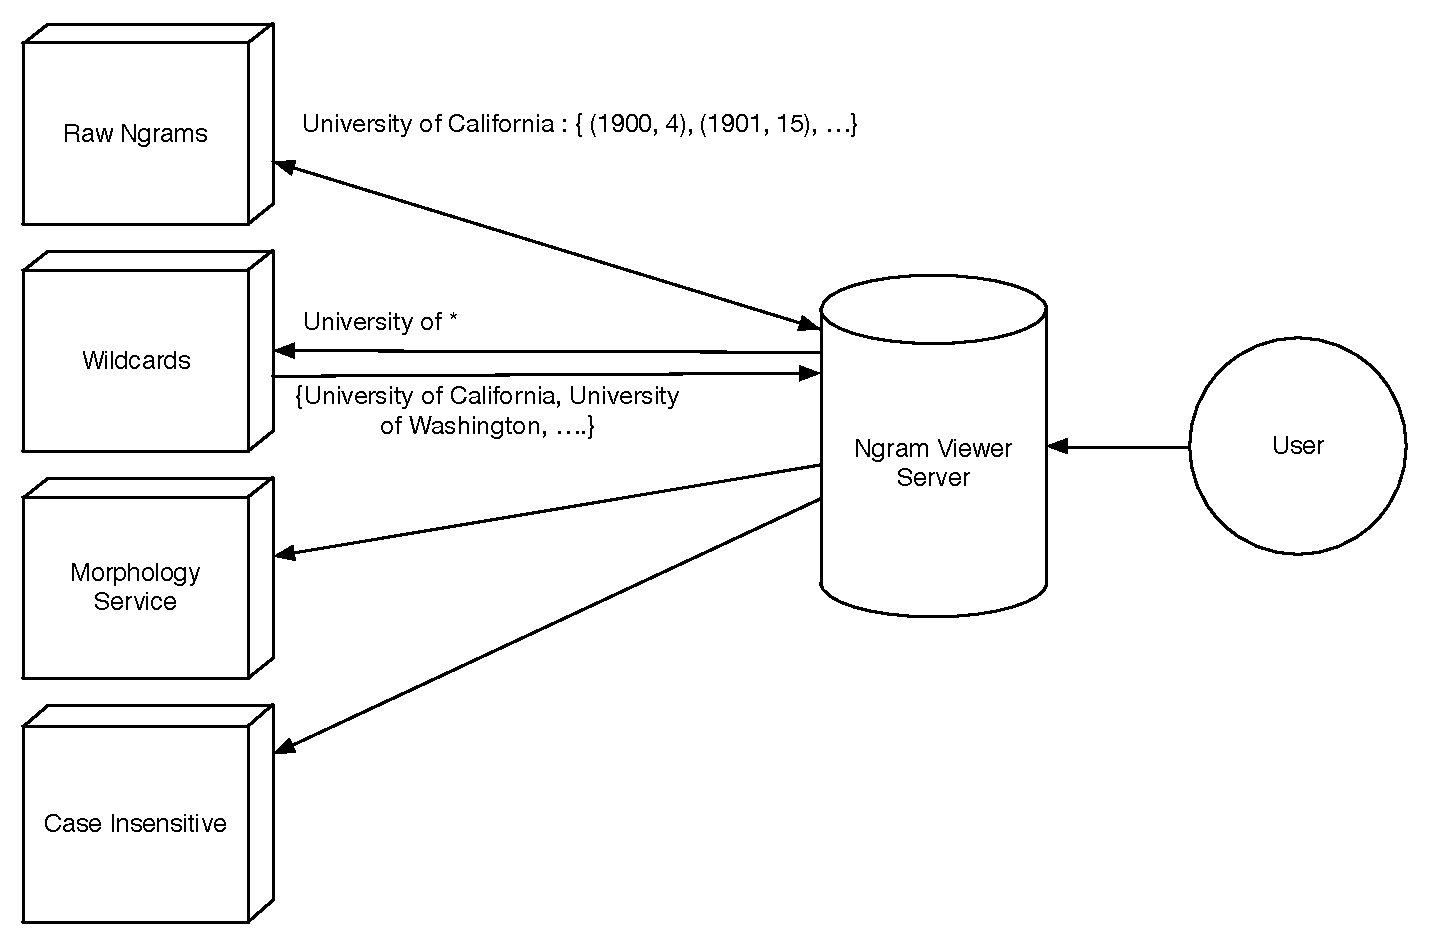
\includegraphics[width=\columnwidth,keepaspectratio=true]{system_architecture}
\caption{\label{fig:architecture}Diagram of new system architecture. The objects with dotted lines show the added tables.}
\end{figure}

\begin{table*}[!t]
\small
\centering
\begin{tabular}{|c|c|}
\hline
\textbf{Query}	& \textbf{Possible Replacements}	\\ \hline \hline
\query{a * man}				& \query{a young man, a good man, a kind man, a wild man	}	\\ \hline
\query{booked=>*\_NOUN}	& 
\begin{tabular}[c]{@{}c@{}} \query{ booked=>flight\_NOUN, booked=>passage\_NOUN, }\\\query{booked=>room\_NOUN, booked=>eat\_NOUN}  \end{tabular} \\ \hline
\query{John said\_INF		}	& \query{John says, John said, John say, John saying} \\ \hline
\query{book\_INF\_NOUN		}	& \query{book, books     } \\ \hline
\begin{tabular}[c]{@{}c@{}} \query{the cook} (case insensitive)\end{tabular} & \query{THE COOK, the cook, The Cook, the Cook, The cook  } 	  \\ \hline
\end{tabular}
\caption{\label{tab:wildcard}
Examples of precompiled wildcard, inflection, and capitalization queries.}
\end{table*}

\eat{\begin{figure*}[!t]
\centering
\addtolength{\subfigcapskip}{-0.2cm}
\hspace*{-0.5cm}
\subfigure[]{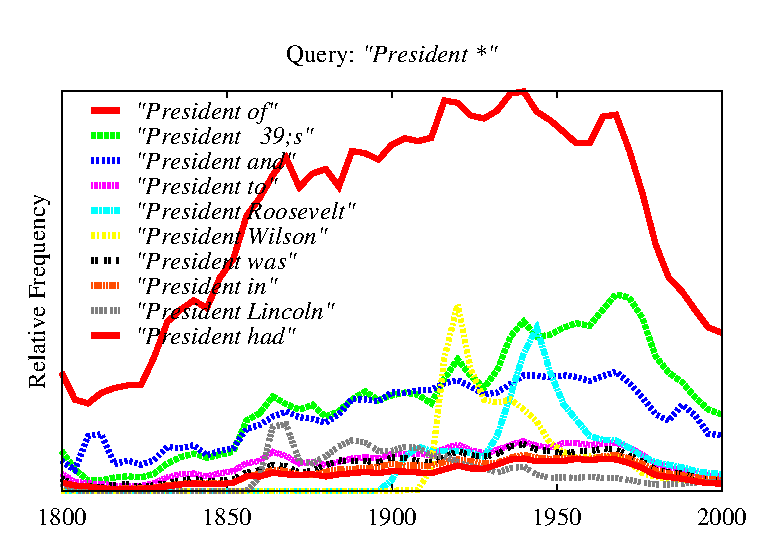
\includegraphics[width=0.49\textwidth]{graphs/president*_all}}
\hspace*{0.1cm}
\subfigure[]{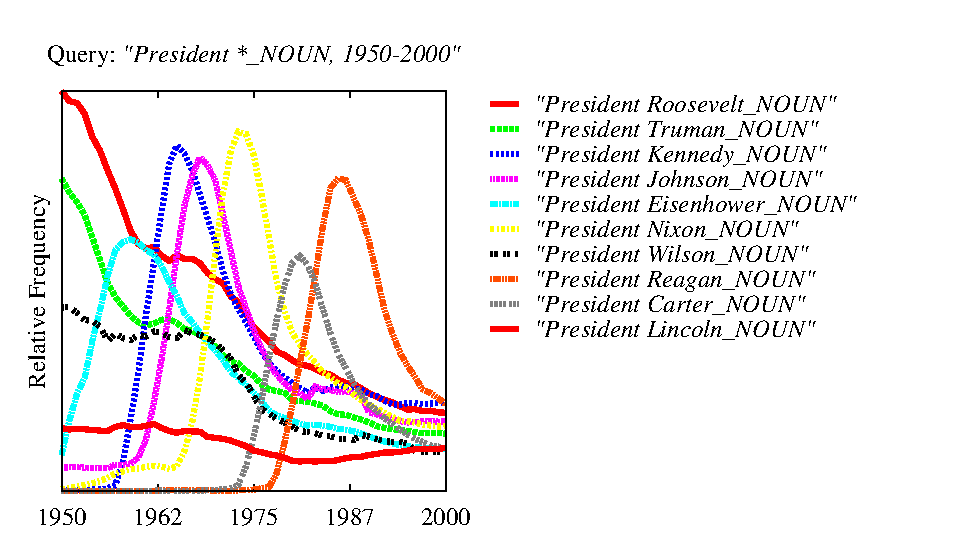
\includegraphics[width=0.49\textwidth]{graphs/President*1950}}

\hspace*{-0.5cm}\vspace*{-0.5cm}
\subfigure[]{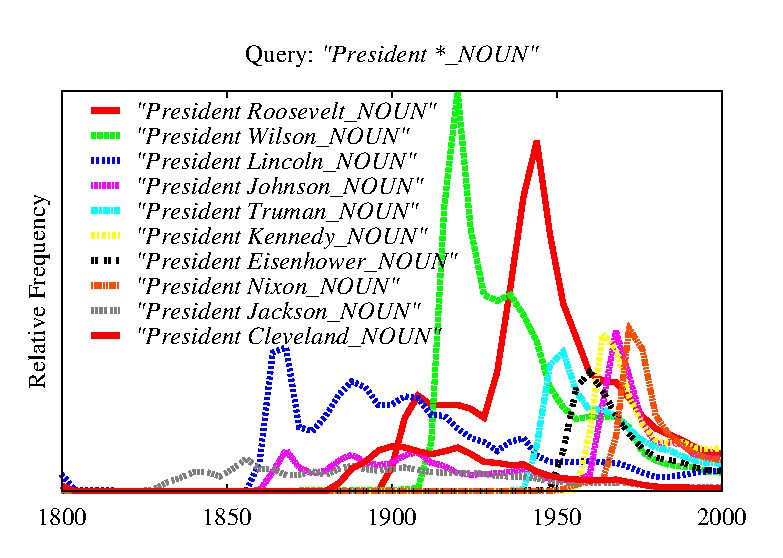
\includegraphics[width=0.69\textwidth]{graphs/President*1800}}
\hspace*{0.1cm}
\parbox[b][]{.28\textwidth}%
{\RawCaption{\caption{\label{fig:presidents}
Specification of a part-of-speech tag along with the wildcard operator results in more
specific results, as shown in (b) and (c).}}}
\end{figure*}}

\begin{figure*}[!t]
\centering
\addtolength{\subfigcapskip}{-0.2cm}
\hspace*{-0.5cm}
\subfigure[]{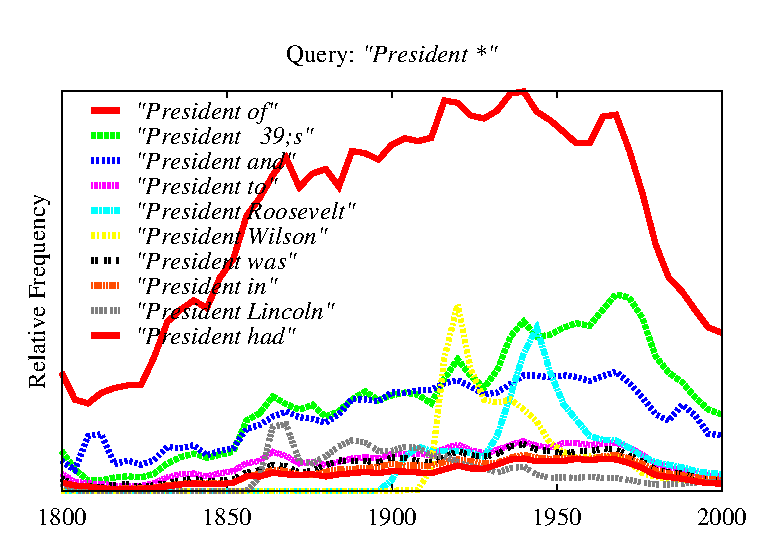
\includegraphics[width=0.49\textwidth]{graphs/president*_all}}
\subfigure[]{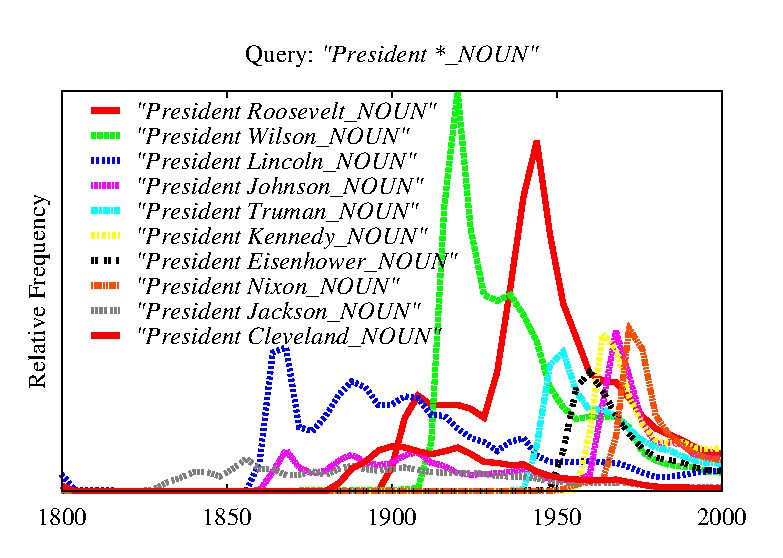
\includegraphics[width=0.49\textwidth]{graphs/President*1800}}
\caption{\label{fig:presidents}
Specification of a part-of-speech tag along with the wildcard operator results in more
specific results, as shown in (b) and (c).}
\end{figure*}

\subsection{Architecture}
The Ngram Viewer provides a lightweight interface to the underlying ngram corpora. In its basic form, user requests are directed through the server to a simple lookup table containing the raw ngrams and their frequencies. This data flow is displayed in the top part of Figure~\ref{fig:architecture} and is maintained for queries that do not involve the new expansion features introduced in this work.

The expansion queries could in principle be implemented by scanning the raw ngrams on the fly and returning the matching subset: to answer the query `\query{President *}', one would need to obtain all bigrams starting with the word \query{President} and extract the most frequent ten. Given the large number of ngrams, such an approach turns out to be computationally very expensive and too slow for an interactive application. We therefore pre-compute intermediate results that can be used to more efficiently retrieve the results for expansion queries. The intermediate results are stored in additional lookup tables (shown at the bottom in Figure~\ref{fig:architecture}). When the user executes an expansion search, the query is first routed to the appropriate lookup table which stores all possible expansions (including expansions that might not appear in the corpus).  These expanded ngrams are then retrieved from the raw ngram table, sorted by frequency and returned to he user.
%For example, the intermediate results table for the morphological variants search contains inflected forms for all unigrams. These inflected forms are substituted for the selected query term and the resulting ngram is looked up in the raw ngram table.
We describe the intermediate results tables and how they are generated in the next section.

Note that we only support one expansion per query ngram. This is needed in order to avoid the combinatorial explosion that would result from mixing multiple expansions in a query.


\section{New Features}
\label{sec:features}
The three new search features are implemented via the same two-step approach. As shown in Figure~\ref{fig:architecture}, we maintain three new lookup tables that hold intermediate results needed for efficiently retrieving the necessary expansions. Below, we describe how these intermediate results are generated and how they are used to retrieve the final results.

\subsection{Wildcards}
\label{sec:wildcards}
	We support the use of wildcards by utilizing an additional database that stores the most frequent expansions of queries to the ngram corpus. This wildcard database is created as a pre-compilation step when creating the Ngram Corpus from the Google Books data. When a new ngram is created, one word or tag at a time is replaced with the wildcard symbol, `\query{*}', creating a wildcard query. The query becomes a key in a string-indexed lookup table, and the original ngram is added to a list of ngrams which are its values. As mentioned above, due to space considerations we were not able to store all possible expansions for every wildcard ngram we precomputed. Also, we could not precompute a perfect set of the top 10 ngrams for every possible year range, while this would require intermediate storage space on the order discussed above, as well as the computation time to calculate the top 10 for $\frac{n(n+1)}{2}$ time periods for each wildcard (where $n$ is the full year range of the Ngram Corpus). For example the query `\query{the *}' has 2,353,960 expansions, making it to both impractical store all its replacements and impossible to serve an exact computation at runtime. Instead we estimate the top 10 during the creation of wildcard ngrams, by limiting the number of expansions to the top ten for every year. We gather these top 10 lists into a union and map the raw ngrams to the wildcard ngram string in our table. 
	
	During this process, we filter punctuation from consideration as a valid expansion because in practice punctuation returns uninteresting results. Note that it may be useful to specify a particular POS tag with the wildcard operator (e.g., `\query{*\_NOUN}') to retrieve more specific results. At runtime, union of expansion ngrams is processed for the specific year range requested and the top ten results are returned. For examples of expansions see Table \ref{tab:wildcard}. 

\subsection{Morphological Inflections}\label{sec:morph}
Inflections of words in search queries are handled using an interface that can provide morphological variations of words for different syntactic categories. This interface makes use of Wiktionary.\footnote{See \url{http://www.wiktionary.org/}.} When a word's
morphological variations are present in the resource, they are retrieved from it; if a word is missing or its entries are incomplete, we use the approach of \newcite{durrett2013supervised} to predict the missing forms.\footnote{As this type of search request utilizes an interface which may be updated with new additions to Wiktionary, results for a particular query may change over time.} Unlike wildcard substitutions, there is no need for pre-computation; given a query with the keyword \textsf{\textsc{\_inf}} attached to a word (e.g., `\query{John said\_INF}'), we get the counts of all the ngrams that start with `John' and have the morphological inflections of the root form `say' as its second word in the Ngram Corpus. During experimentation, we noticed that there can be more than 10 results returned per query, especially for morphologically rich languages like Russian, unlike the wildcard search feature. Therefore we have updated the user interface to better deal with more data lines (\S\ref{sec:usecases}). We do not allow the combination of morphological inflections with wildcards and/or capitalization searches because it slows down the retrieval process.

\subsection{Capitalization}
Capitalization searches are enabled by selecting a case-insensitive check box on the new interface. These queries, like the wildcards, are referenced to a separate database that contains a mapping of different case combinations to the ngram string in lowercase. All possible variations in case are captured by a process similar to building the wildcard expansion table. To create the capitalization lookup table, we map all raw ngrams in a precomputation step to their lowercased forms. During experimentation, we noticed that often there are many capitalization variants of a given query for which the ngram counts are negligible; hence, to keep our results meaningful, we filter out all variants that have a cumulative count of less than 1\% of the most frequent variant for a given year range.

\eat{\section{User Interface}
\label{sec:interface}}

\eat{\begin{figure}[!t]
\centering
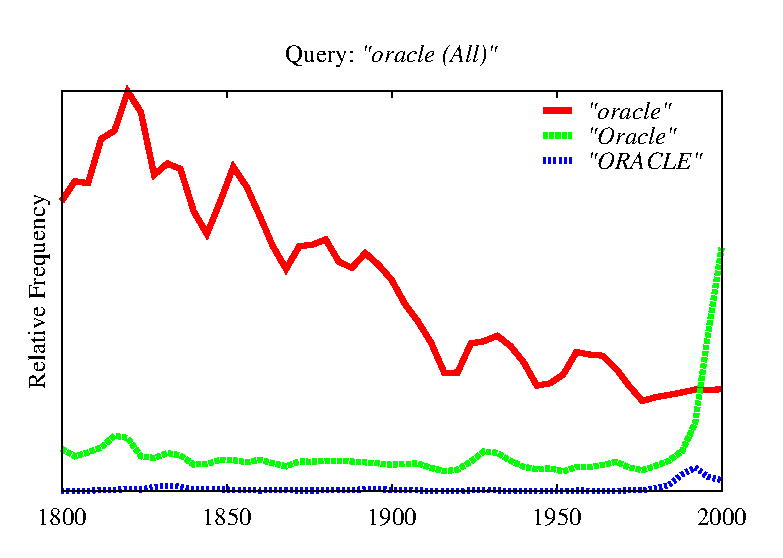
\includegraphics[width=\columnwidth]{graphs/oracle}
\caption{\label{fig:oracle} Discovery of Capitalization usage.
\vspace*{-1.5em}}
\end{figure}}


\section{Use Cases}
\label{sec:usecases}

The previous version of the Ngram Viewer introduced specific search features that could exploit POS tag and syntactic dependency annotations in the Ngram Corpus \cite{lin2012syntactic}. The three features introduced in this paper continue this trend of specialization, but also provide the ability to group similar searches, preventing the need for overly verbose queries. Below we examine example uses of the new features in isolation, and combined with the features already present. We show queries to highlight specific usages that we feel users will find the most useful, but wish to leave the analysis of the results to the experts.

\begin{figure*}[t]
\subfigure[All expansions.]{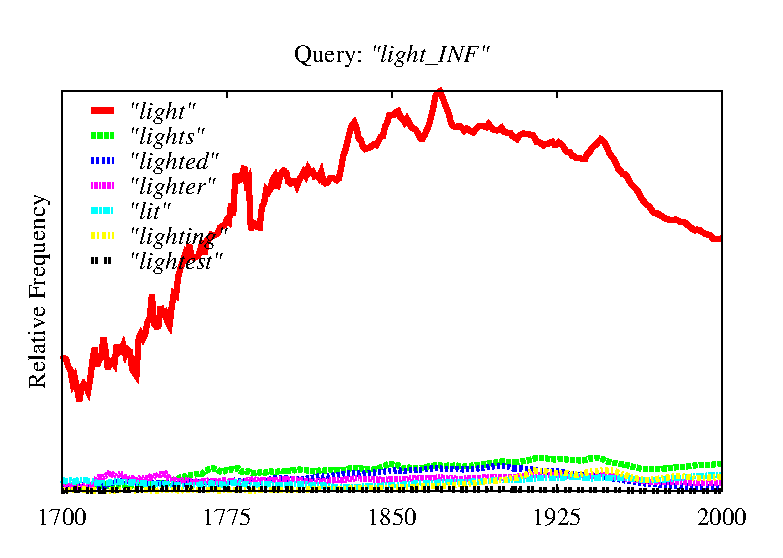
\includegraphics[width=.48\textwidth]{graphs/light_INF}}
\subfigure[Verbs only.]{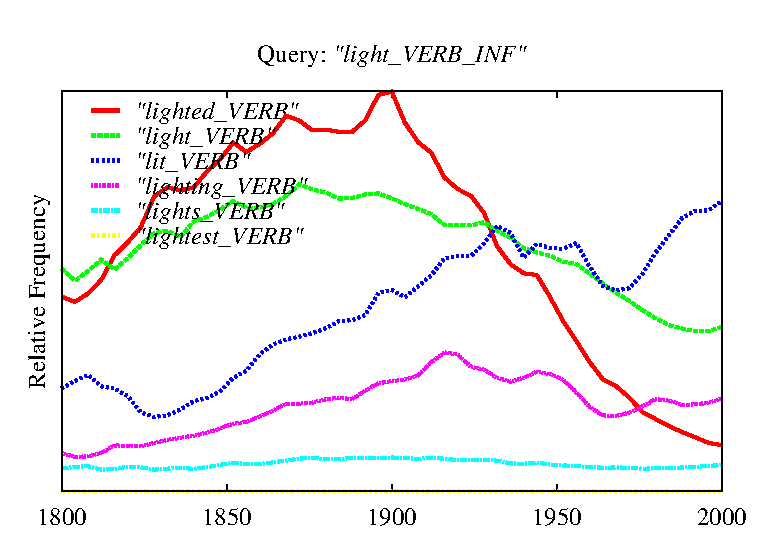
\includegraphics[width=.48\textwidth]{graphs/light_INF_VERB}}
\vspace*{-1em}
\caption{\label{fig:light} Comparison of specification of POS tag in wildcard search.}
\end{figure*}

\begin{table*}[ht]
\small
\centering
\begin{tabular}{|c|c|c|c|c|c|c|c|c|c|}
\hline
\textbf{English} & \textbf{American} & \textbf{British} & \multirow{2}{*}{\textbf{German}} & \multirow{2}{*}{\textbf{French}} & \multirow{2}{*}{\textbf{Russian}} & \multirow{2}{*}{\textbf{Italian}} & \textbf{Chinese} & \multirow{2}{*}{\textbf{Spanish}} & \multirow{2}{*}{\textbf{Hebrew}} \\
\textbf{(All)} &  \textbf{English} & \textbf{English} & & & & &  \textbf{(Simplified)} & &  \\
\hline
\query{drinks} & \query{drinks} & \query{drinks} & \query{trinkt} & \query{boit} & \textcyr{p\char126et} & \query{beve} & \begin{CJK}{UTF8}{gbsn}  喝 \end{CJK} & \query{bebe} & \heb{שותה}\\
\hline \hline
\query{water}&\query{water}&\query{water}&\query{Wein}  &\query{vin}  &\textcyr{on}       &\query{vino}    &\begin{CJK}{UTF8}{gbsn}酒  \end{CJK}&\query{agua}   &\heb{יין}\\
\query{wine} &\query{wine} &\query{wine} &\query{Wasser}&\query{eau}  &\textcyr{cha{\u i}}&\query{acqua}   &\begin{CJK}{UTF8}{gbsn}茶  \end{CJK}&\query{sangre} &\heb{מים}\\
\query{man}  &\query{blood}&\query{blood}&\query{Blut}  &\query{sang} &\textcyr{vodu}     &\query{sangue}  &\begin{CJK}{UTF8}{gbsn}水  \end{CJK}&\query{vino}   &\heb{ה}  \\
\query{blood}&\query{man}  &\query{man}  &\query{Bier}  &\query{verre}&\textcyr{On}       &\query{latte}   &\begin{CJK}{UTF8}{gbsn}咖啡\end{CJK}&\query{vaso}   &\heb{כוס}\\
\query{tea}  &\query{tea}  &\query{tea}  &\query{Kaffee}&\query{L'}   &\textcyr{vino}     & \query{caff\'e}&\begin{CJK}{UTF8}{gbsn}人  \end{CJK}&\query{cerveza}&\heb{אדם}\\\hline 
\end{tabular}
\caption{\label{tab:drink} Comparison of top dependencies from `drink' in all corpora. Queries were initiated by translation from `drinks' using Google Translate, and entered into the Ngram Viewer using the format \query{(drink)=>*\_NOUN}. Therefore the queries may not agree on tense/aspect/gender, so forth, across the different languages.}
\end{table*}

Before our additions to the Ngram Viewer, a user could manually create query sets resulting identical charts, but often would have to examine the ngram data to carefully craft them. For example, Figure~\ref{fig:manual} shows a manually created query set searching for specific presidents; Figure \ref{fig:presidents}(b) on the other hand, is a single wildcard query over the same time range; it automatically retrieves the 10 most popular presidents and shows additional trends that would have required extra work on behalf of the user to generate.

The wildcard feature used on its own can be a powerful tool for the analysis of top expansions for a certain context.  Although compelling in isolation, we have found more interesting trends when the wildcard feature is combined with POS tags. The user can attach an underscore and POS tag to either a wildcard-based or inflection based query to specify that the expansions returned should be of a specific part of speech. Compare the utility of the generic wildcard and a search with a noun part-of-speech specification in a query examining president names, `\query{President *}'/`\query{President *\_NOUN}' shown in Figure \ref{fig:presidents}. The former gives a mixture of prepositions, particles, and verbs along with names of presidents, and because the latter specifies the noun tag, the top expansions turn out to be names and more in line with the intention of the search. Also, note in Figure \ref{fig:presidents} the difference in expansions that searching over two different time ranges provides.

It is worth noting that the newly introduced features could result in many lines in the resulting chart as mentioned in \S\ref{sec:morph}; hence, we have updated the Viewer's user interface to handle several retrieved ngrams. Interactive functionality allows the user to highlight a line by hovering over it, keep that focus by left clicking, and clear all focused lines by double clicking. A right click on any of the expansions returned by an issued query combines them into the year-wise sum total of all the expansions. We added another feature to the interface that creates static URLs maintaining all the raw ngrams retrieved from any query. This prevents statically linked charts from changing over time, and allowing for backwards compatibility.

One of the primary benefits of searching with the capitalization feature is the combination of multiple searches in one, which allows the user to compare completely case-insensitive usages of two different phrases. An alternative use is in Figure~\ref{fig:examples}(c), where using capitalization searches allows for immediate identification of changing orthographic usage of a word or phrase, which in this case shows the arrival of F. Scott Fitzgerald in the early to mid 20th century as well as the rise in popularity of the camelCase variety of his surname at the turn of the century.

Searches using the inflections can be useful for the same reasons detailed for capitalization searches, but compare changes in spelling. This feature becomes particularily useful for the analysis of irregular verbs, where the query can return both the regular and irregular forms of a verb if they are statistically significant.


\section{Conclusions}
We have presented a new version of the Ngram Viewer with some new functionality. With the introduction of these new features, users can perform more powerful searches that show trends which were not possible to extract from earlier versions of the Viewer. The new features have been highlighted in a recent article by the Atlantic, as well on various blogs.
We hope the presented functionalitied of the Viewer will help uncover trends and patterns not readily apparent in the Ngram Corpus.

\eat{\jmcomment{Blog posts/entries from the internet:
http://sciencerefinery.com/2013/10/28/google-ngram-viewer-now-more-powerful-than-ever/
http://www.devingriffiths.com/google-books/google-n-gram-studies/
http://languagelog.ldc.upenn.edu/nll/?p=8472
http://www.textualscholarship.nl/?p=14051}}

\eat{\section{Acknowledgements}
We would like to thank John DeNero, ...}

\bibliographystyle{acl}
\bibliography{acl2014}


\eat{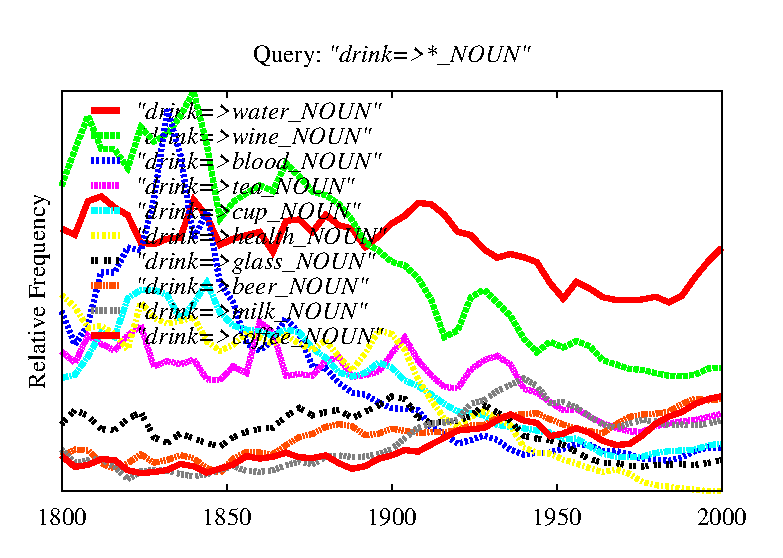
\includegraphics[width=.48\textwidth]{graphs/drink}
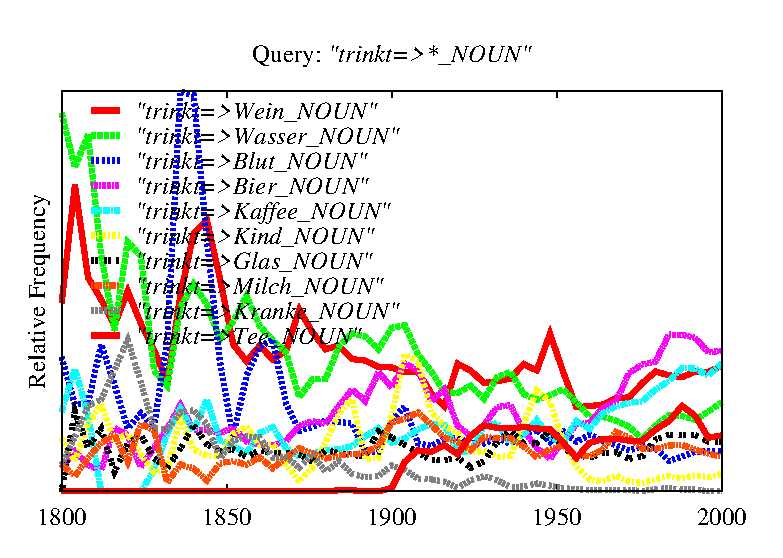
\includegraphics[width=.48\textwidth]{graphs/drink_GER}
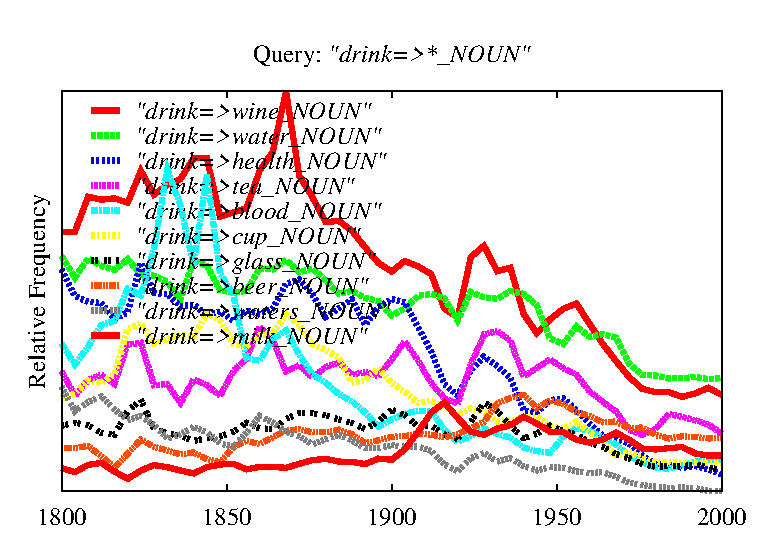
\includegraphics[width=.48\textwidth]{graphs/drink_UK}
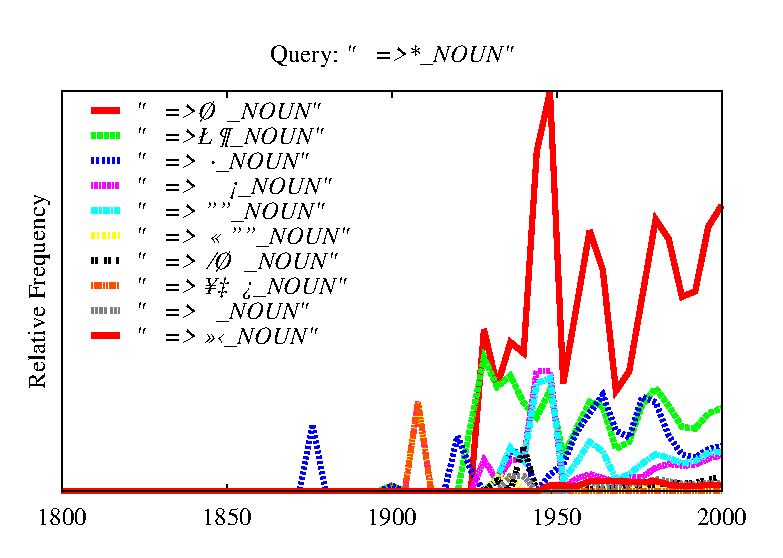
\includegraphics[width=.48\textwidth]{graphs/drink_CHI}
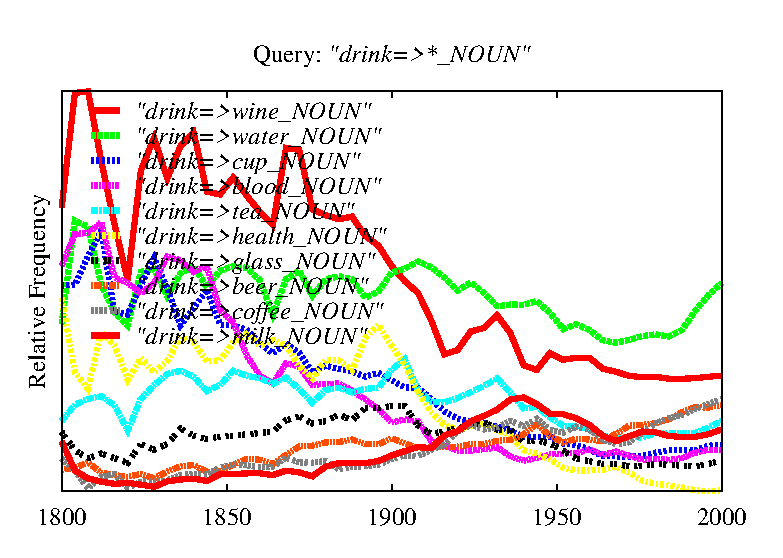
\includegraphics[width=.48\textwidth]{graphs/drink_USA}
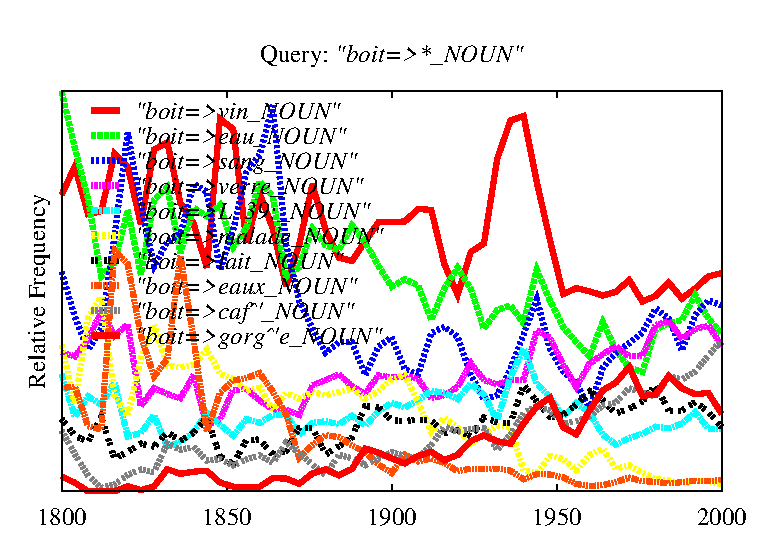
\includegraphics[width=.48\textwidth]{graphs/drink_FRE}
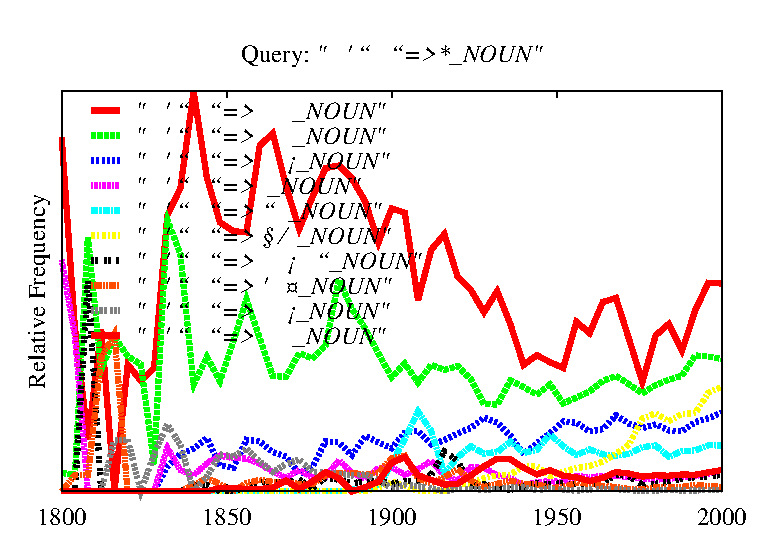
\includegraphics[width=.48\textwidth]{graphs/drink_HEB}
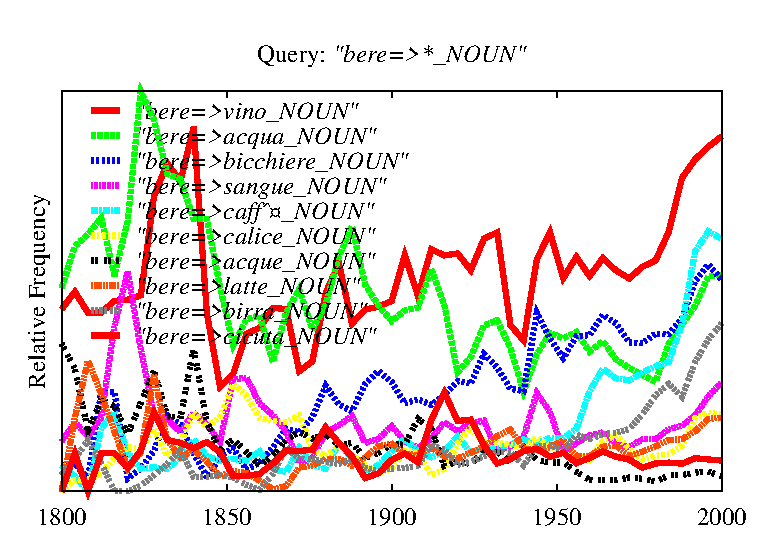
\includegraphics[width=.48\textwidth]{graphs/drink_ITA}
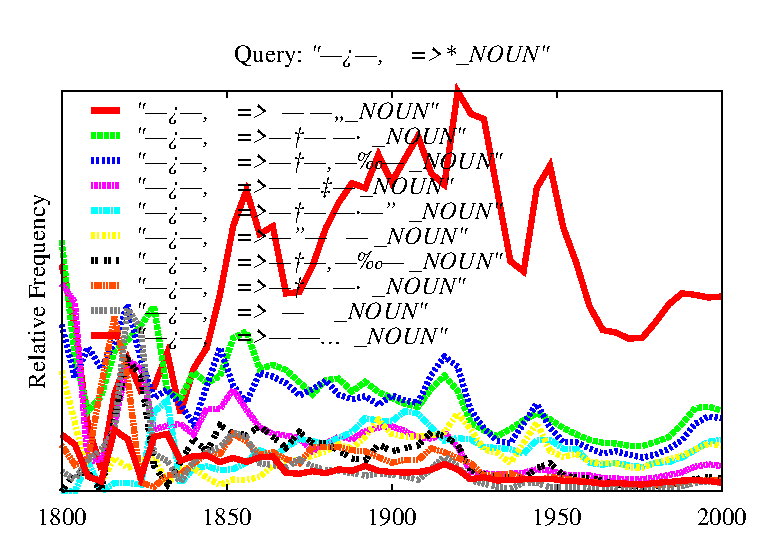
\includegraphics[width=.48\textwidth]{graphs/drink_RUS}
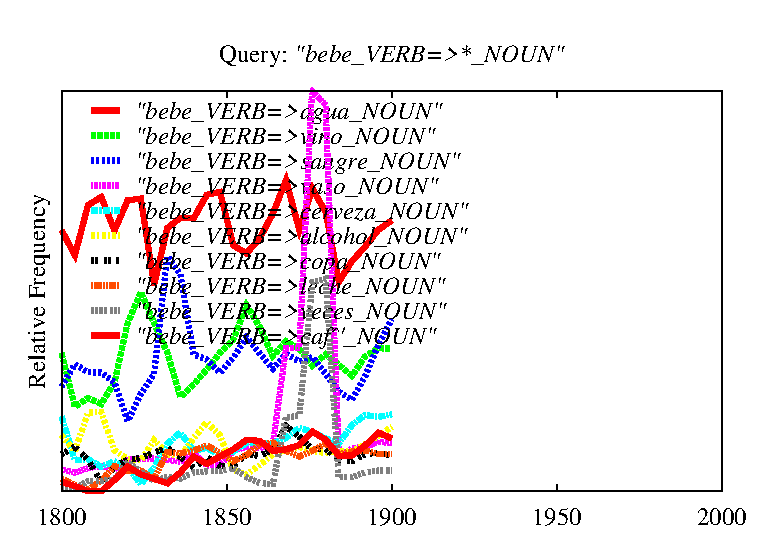
\includegraphics[width=.48\textwidth]{graphs/drink_SPA}}


\end{document}
